\chapter*{Bases de données relationnelles}
\setcounter{chapter}{1}
Pour bien commencer ce cours, nous devons comprendre la notion de base de données et la préciser petit à petit.
\begin{Comprendre}Pour commencer, regardez la vidéo d'Informatique Sans Complexe qui introduit le concept de base de données.~\url{https://www.youtube.com/watch?v=D5dE_XN8b6w}
\end{Comprendre}
\begin{Definition}[Base de données]
Une base de données permet de stocker et de retrouver des données structurées, semi-structurées ou des données brutes, souvent en rapport avec un thème ou une activité. Celles-ci peuvent être de natures différentes et plus ou moins reliées entre elles.\\
\textit{source : Wikipédia}
\end{Definition}

Une base de données permet de centraliser les données pour faciliter leur stockage, leur collecte et leur utilisation par différents services ou utilisateurs.

En vérité, il n'existe pas de définition unique du mot "base de données". En général, les bases de données sont des systèmes de gestion de l'information. Elles peuvent être plus ou moins structurées. Lorsque les données sont structurées, elles peuvent aider les utilisateurs et les ordinateurs à travailler plus efficacement avec les données. \\
Une base donnée doit satisfaire 4 opérations primaires sur les données (on parle de \motcle{transactions}), que l'on résume avec l'acronyme~\motcle{CRUD} pour :
\begin{center}
\begin{description}
    \item[CREATE] : Ajouter des données
    \item[READ] : Lire les données
    \item[UPDATE] : Mettre à jour les données
    \item[DELETE] : Supprimer des données
\end{description}
\end{center}
Dans un monde idéal, les transactions doivent satisfaire 4 propriétés importantes, on parle du modèle~\motcle{ACID} pour :
\begin{description}
    \item[Atomicité] : Tout changement est fait du début à la fin.
    \item[Cohérence] : Les contraintes sont toujours respectées.
    \item[Isolation] : Des transactions exécutées en même temps ne se perturbent pas : le résultat est le même que si elles étaient faites l'une après l'autre.
    \item[Durabilité] : Les données continuent d'être conservées même en cas de défaillance.
\end{description}
%


Les bases de données \motcle{relationnelles} sont le type de base de données le plus connu. Elles sont constituées de tableaux,  qui ressemblent beaucoup à des feuilles de calcul (comme sur Excel ou libre office Calc par exemple). Chaque colonne du tableau porte un nom et un type de données (texte, nombre, etc.), et chaque ligne du tableau correspond à un enregistrement spécifique. On appelle \motcle{relation} le nom du tableau, \motcle{attribut} le nom des colonnes et chaque ligne est un \motcle{enregistrement} de la base de données. 


La partie "relationnelle" s'accompagne de règles spécifiques sur la manière de connecter les données entre les différentes tables.
L'ensemble de ces règles est défini grâce au \motcle{modèle relationnel}.

\begin{Comprendre}
    \begin{center}
        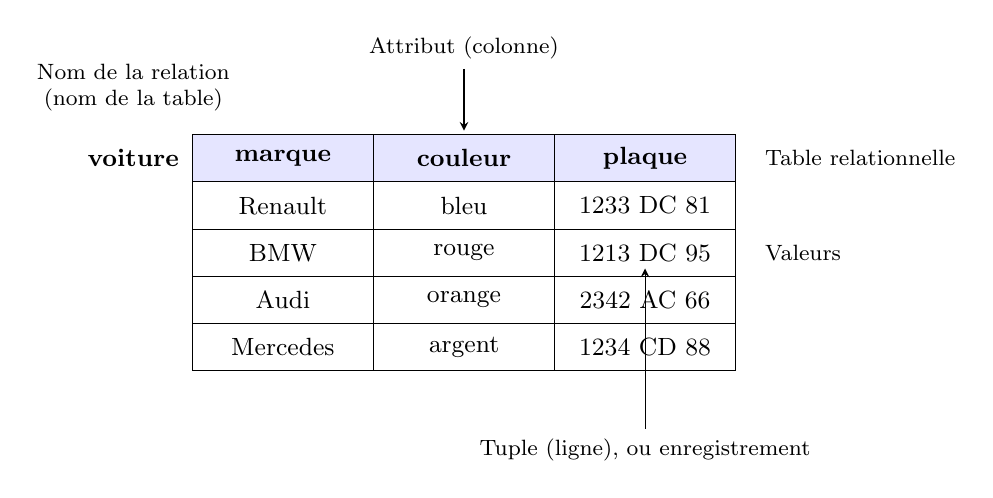
\begin{tikzpicture}[x=1cm,y=1cm,c/.style={draw,minimum height=0.6cm,minimum width=2.3cm,font=\small},h/.style={c,fill=blue!10,font=\small\bfseries},n/.style={font=\footnotesize,align=center,text=black}]
\node[h] at (0.0,0.0){marque};
\node[h] at (2.3,0.0){couleur};
\node[h] at (4.6,0.0){plaque};
\node[c] at (0.0,-0.6){Renault};
\node[c] at (2.3,-0.6){bleu};
\node[c] at (4.6,-0.6){1233 DC 81};
\node[c] at (0.0,-1.2){BMW};
\node[c] at (2.3,-1.2){rouge};
\node[c] at (4.6,-1.2){1213 DC 95};
\node[c] at (0.0,-1.8){Audi};
\node[c] at (2.3,-1.8){orange};
\node[c] at (4.6,-1.8){2342 AC 66};
\node[c] at (0.0,-2.4){Mercedes};
\node[c] at (2.3,-2.4){argent};
\node[c] at (4.6,-2.4){1234 CD 88};
\node[n] (rel) at (-1.9,0.9){Nom de la relation\\(nom de la table)};\node[font=\small\bfseries] at (-1.9,0){voiture};
\node[n] (att) at (2.3,1.4){Attribut (colonne)};\draw[->,>=stealth] (att.south)--(2.3,0.35);
\node[n] (tup) at (4.6,-3.7){Tuple (ligne), ou enregistrement};\draw[->,>=stealth] (tup.north)--(4.6,-1.4);
\node[n,anchor=west] at (6.0,-1.2){Valeurs};\node[n,anchor=west] at (6.0,0){Table relationnelle};
\end{tikzpicture}
    \end{center}
    Par exemple, la base de données ci-dessus contient de l'information sur des voitures : leur marque, couleur et plaque. Le premier enregistrement est une Renault, bleue dont la plaque est : 1233 DC 81
\end{Comprendre}

\section{Modèle relationnel}
Pour la suite du cours, nous suivrons comme fil conducteur la base de données SQL Murder Mystery (\url{https://mystery.knightlab.com/walkthrough.html}). 
Le Mystère du Meurtre SQL est conçu à la fois comme une leçon autodidacte pour apprendre les concepts et les commandes SQL et comme un jeu amusant pour les utilisateurs SQL expérimentés afin de résoudre un crime intrigant.\\

\begin{center}
    {\large Notre objectif de fin de chapitre : savoir interroger cette base pour résoudre l'enquête sur le site du jeu.}\\
\end{center}

De manière générale, on peut représenter le modèle relationnel sous forme de diagramme. C'est une représentation \textbf{visuelle} des relations entre toutes les tables d'une base de données. Vous trouverez ci-dessous le diagramme de notre base de données SQL Murder Mystery. Le diagramme montre que chaque table a un nom (en haut de la boîte, en gras), une liste de noms de colonnes (à gauche) et leurs types de données correspondants (à droite, en majuscules). Le dernier mot de chaque ligne indique le rôle de la colonne : PK pour la \motcle{clé primaire} de la table, FK pour une \motcle{clé étrangère}. Si deux tables sont liées, elles sont reliées par une flèche, qui va de la clé étrangère vers la table référencée.

\begin{Definition}[Clé primaire]
Dans une base de données relationnelle, une clé primaire est la donnée qui permet d'identifier de manière \textbf{unique} un enregistrement dans une table. Deux lignes distinctes de la table ne peuvent pas avoir les mêmes valeurs dans les colonnes définies comme clé primaire.
\end{Definition}

\begin{Definition}[Clé étrangère]
Une clé étrangère, dans une base de données relationnelle, identifie une colonne d'une table comme référençant une colonne d'une autre table (la table référencée). La contrainte de clé étrangère garantit que les valeurs de chaque ligne de la table référençant existent dans la table référencée : ainsi une ligne de la table référençant ne peut pas contenir un ensemble de valeurs qui n'existe pas dans la table référencée. 
\end{Definition}

\begin{figure}
    \centering
    \resizebox{\linewidth}{!}{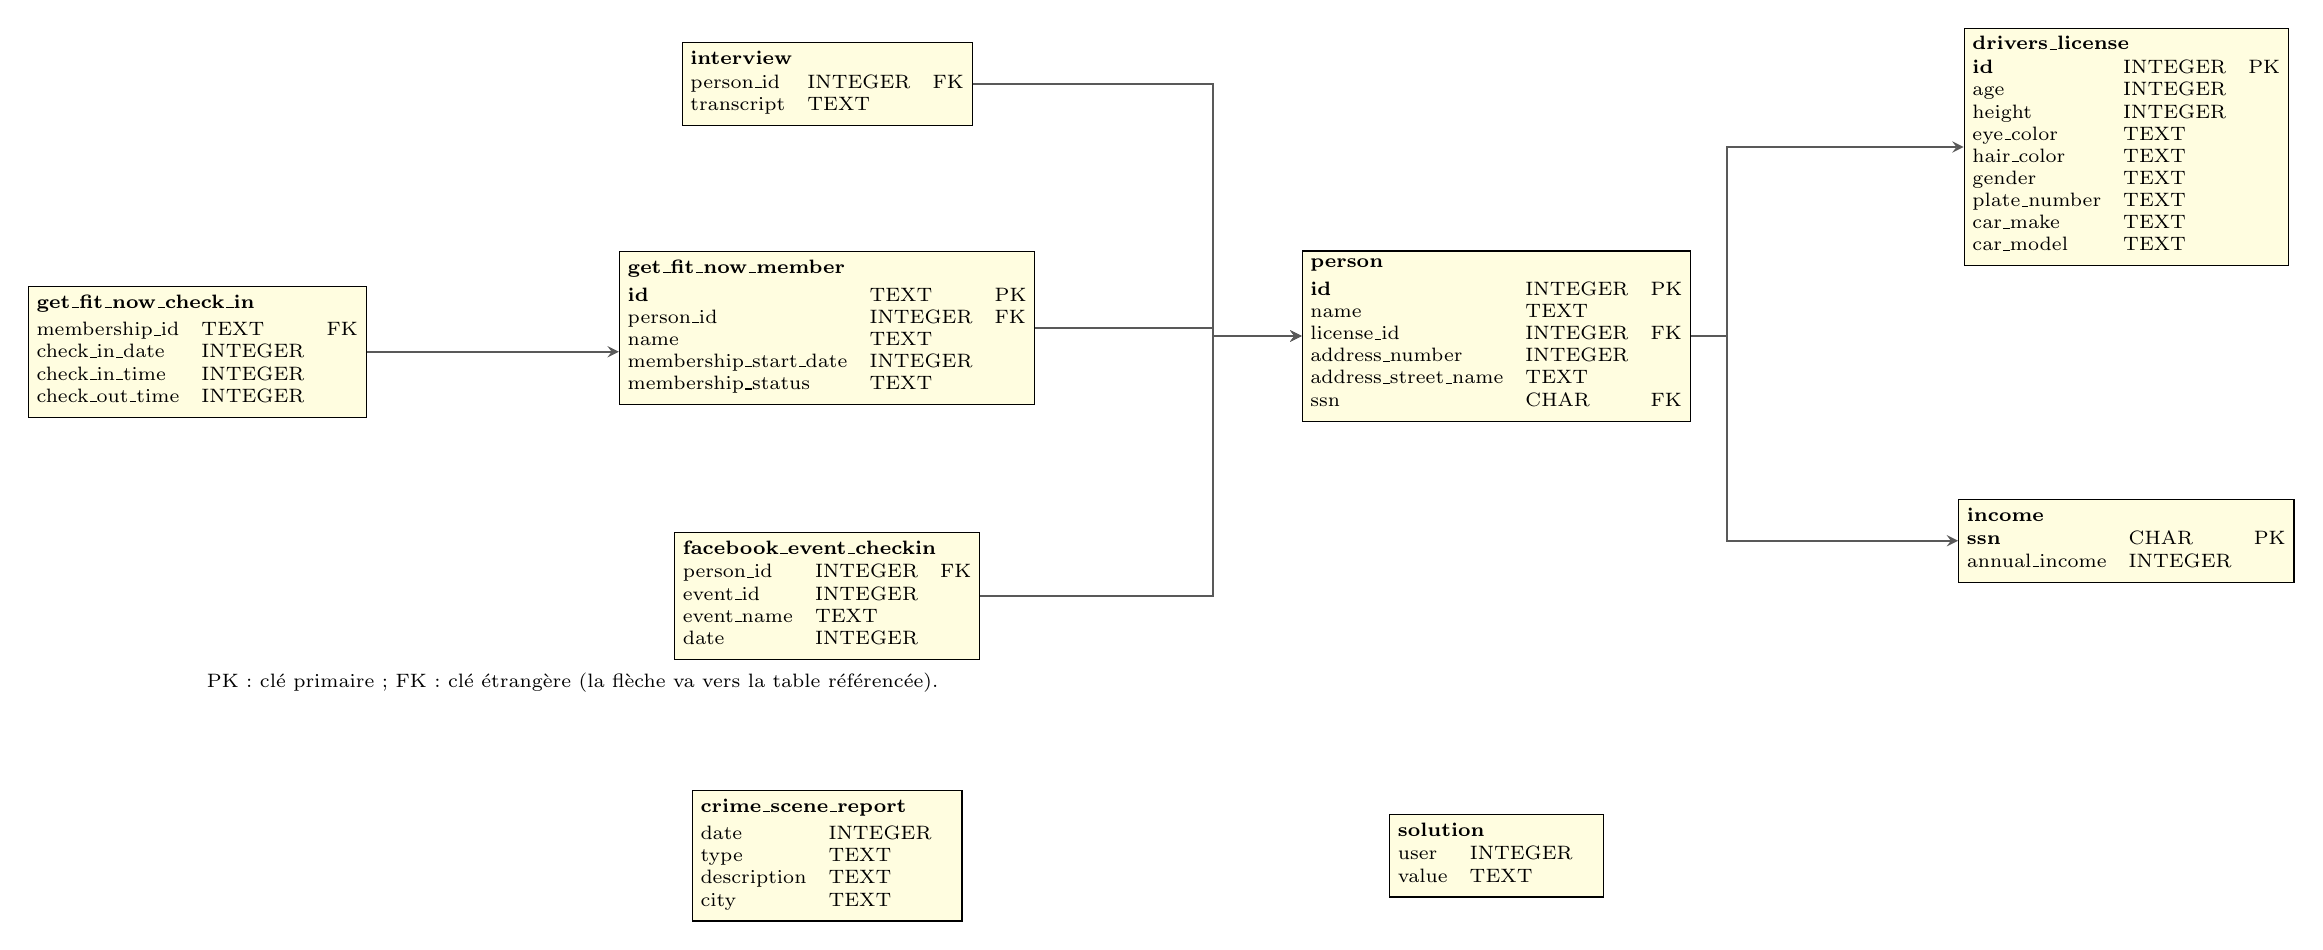
\begin{tikzpicture}[x=1cm,y=1cm,tbl/.style={draw,fill=yellow!12,inner sep=3pt,font=\scriptsize,align=left},fk/.style={->,>=stealth,thick,gray!70!black}]
\node[tbl] (get_fit_now_check_in) at (0.0,0.0) {\textbf{get\_fit\_now\_check\_in}\\[2pt]\begin{tabular}{@{}l@{\quad}l@{\quad}l@{}}
membership\_id & TEXT & FK\\
check\_in\_date & INTEGER & \\
check\_in\_time & INTEGER & \\
check\_out\_time & INTEGER & \\
\end{tabular}};
\node[tbl] (interview) at (8.0,3.4) {\textbf{interview}\\[2pt]\begin{tabular}{@{}l@{\quad}l@{\quad}l@{}}
person\_id & INTEGER & FK\\
transcript & TEXT & \\
\end{tabular}};
\node[tbl] (get_fit_now_member) at (8.0,0.3) {\textbf{get\_fit\_now\_member}\\[2pt]\begin{tabular}{@{}l@{\quad}l@{\quad}l@{}}
\textbf{id} & TEXT & PK\\
person\_id & INTEGER & FK\\
name & TEXT & \\
membership\_start\_date & INTEGER & \\
membership\_status & TEXT & \\
\end{tabular}};
\node[tbl] (facebook_event_checkin) at (8.0,-3.1) {\textbf{facebook\_event\_checkin}\\[2pt]\begin{tabular}{@{}l@{\quad}l@{\quad}l@{}}
person\_id & INTEGER & FK\\
event\_id & INTEGER & \\
event\_name & TEXT & \\
date & INTEGER & \\
\end{tabular}};
\node[tbl] (person) at (16.5,0.2) {\textbf{person}\\[2pt]\begin{tabular}{@{}l@{\quad}l@{\quad}l@{}}
\textbf{id} & INTEGER & PK\\
name & TEXT & \\
license\_id & INTEGER & FK\\
address\_number & INTEGER & \\
address\_street\_name & TEXT & \\
ssn & CHAR & FK\\
\end{tabular}};
\node[tbl] (drivers_license) at (24.5,2.6) {\textbf{drivers\_license}\\[2pt]\begin{tabular}{@{}l@{\quad}l@{\quad}l@{}}
\textbf{id} & INTEGER & PK\\
age & INTEGER & \\
height & INTEGER & \\
eye\_color & TEXT & \\
hair\_color & TEXT & \\
gender & TEXT & \\
plate\_number & TEXT & \\
car\_make & TEXT & \\
car\_model & TEXT & \\
\end{tabular}};
\node[tbl] (income) at (24.5,-2.4) {\textbf{income}\\[2pt]\begin{tabular}{@{}l@{\quad}l@{\quad}l@{}}
\textbf{ssn} & CHAR & PK\\
annual\_income & INTEGER & \\
\end{tabular}};
\node[tbl] (crime_scene_report) at (8.0,-6.4) {\textbf{crime\_scene\_report}\\[2pt]\begin{tabular}{@{}l@{\quad}l@{\quad}l@{}}
date & INTEGER & \\
type & TEXT & \\
description & TEXT & \\
city & TEXT & \\
\end{tabular}};
\node[tbl] (solution) at (16.5,-6.4) {\textbf{solution}\\[2pt]\begin{tabular}{@{}l@{\quad}l@{\quad}l@{}}
user & INTEGER & \\
value & TEXT & \\
\end{tabular}};
\draw[fk] (get_fit_now_check_in.east) -- (get_fit_now_member.west|-get_fit_now_check_in.east);
\draw[fk] (get_fit_now_member.east) -- (12.9,0 |- get_fit_now_member.east) |- (person.west);
\draw[fk] (interview.east) -- (12.9,0 |- interview.east) |- (person.west);
\draw[fk] (facebook_event_checkin.east) -- (12.9,0 |- facebook_event_checkin.east) |- (person.west);
\draw[fk] (person.east) -- ++(0.45,0) |- (drivers_license.west);
\draw[fk] (person.east) -- ++(0.45,0) |- (income.west);
\node[font=\scriptsize,anchor=west] at (0,-4.2) {PK : clé primaire ; FK : clé étrangère (la flèche va vers la table référencée).};
\end{tikzpicture}}
    \captionsetup{labelformat=empty}
    \caption{Schéma relationnel de la base de données SQL Murder Mystery.}
    \label{fig:SQLmystery-table}
\end{figure}

\subsection*{Le modèle relationnel de SQL Murder Mystery }
Pour étudier un modèle de base de données, on va toujours chercher les informations suivantes :
\begin{itemize}
\item le nombre de tables et leurs noms,
\item le nombre de colonnes (aussi appelés attributs) pour chaque table, 
\item le type de chaque colonne,
\item le lien entre chacune des tables,
\item les clés primaires et
\item les clés étrangères
\end{itemize}

\begin{Comprendre}
    Passer par un modèle pour une base de données permet de comprendre quelles données sont enregistrées et comment elles sont organisées... Et pas seulement... mais vous découvrirez les autres avantages plus tard dans le cours.
\end{Comprendre}

Étudions de plus près le modèle relationnel de SQL Murder Mystery.\\[-1cm]
\begin{Quizz}
Parmi ces attributs de person, lequel est l'intrus ?
\begin{itemize}
    \renewcommand{\labelitemi}{$\square$}
    \item age
    \item id
    \item name
    \item ssn
\end{itemize}
\end{Quizz}
\begin{Quizz}
Lequel de ces attributs n'est pas une clé primaire ? Notez que la notation avec le point est habituelle. Sa syntaxe est : \textit{table.attribut}. Ainsi \textit{person.id} réfère à l'attribut \textit{id} de la table \textit{person}.
\begin{itemize}
    \renewcommand{\labelitemi}{$\square$}
    \item person.id
    \item drivers\_license.id
    \item interview.person\_id
\end{itemize}
\end{Quizz}
\begin{Quizz}
Lequel de ces attributs n'est pas une clé étrangère ?
\begin{itemize}
    \renewcommand{\labelitemi}{$\square$}
    \item person.license\_id
    \item drivers\_licenses.id
    \item interview.person\_id
\end{itemize}
\end{Quizz}

\begin{Exercise}
 Dans cet exercice  nous n'utilisons que les tables person, interview et drivers\_license. Ci-dessous, chaque ligne d'une table est un tuple de \motcle{valeurs}. L'ensemble des tuples de valeurs constitue-la \motcle{base de données}. C'est le schéma relationnel qui guide leur organisation. \\
 Ainsi la base de données ci-dessous (avant ajout de l'exercice) est constituée de 5 personnes ayant chacune un id, un nom, un identifiant de licence, un numéro d'adresse, un nom de rue de l'adresse et un ssn. Elle est aussi constituée de 2 interviews ayant chacun un numéro de personne et une retranscription (témoignage). Elle est également constituée de permis de conduire (drivers\_license) ayant chacun un identifiant, un âge, une taille, une couleur des yeux, une couleur des cheveux, un genre, un numéro de plaque d'immatriculation, un constructeur de voiture et un modèle de voiture.

\begin{center}

\begin{tabular}{|c c c c c c|}
\hline
\multicolumn{6}{|c|}{\textbf{person}} \\
\hline
    id & name & license\_id & adress\_number & address\_street\_name & ssn \\
    \hline
    \hline
    10000	& Lucien Maradet	& 993845	& 624	& Avenue Bankhall & 747714076\\
10007	& Nolwenn Caldrac	& 861794	& 2791	& Boulevard Gustavus 	& 477972044\\
10010	& Mirko Carvel	& 385336	& 741	& Rue Northwestern	& 828638512\\
10016	& Éva Mosselin	& 431897	& 1987	& Rue Wood Glade	& 614621061\\
54263	& Ioana Gabrelle & 931215	& 1561	& Avenue Murnane & 897118893\\
& & & & &  \\
& & & & &  \\
& & & & &  \\
& & & & &  \\
& & & & &  \\
& & & & &  \\
\hline
\end{tabular}\\
\vspace{25pt}

\begin{tabular}{|c c|}
\hline
\multicolumn{2}{|c|}{\textbf{interview}} \\
\hline
    person\_id & transcript \\
    \hline
    \hline
    10007	& "à 9h j'étais déjà parti au travail" \\
    54263 & "j'ai entendu un cri effroyable"  \\
    &  \\
    &  \\
    &  \\
    &  \\
    &  \\
    &  \\
\hline
\end{tabular}\\
\vspace{25pt}

\begin{tabular}{|c c c c c c c c c|}
\hline
\multicolumn{9}{|c|}{\textbf{drivers\_license}} \\
\hline
    id & age & height & eye\_color & hair\_color & gender & plate\_number & car\_make & car\_model \\
    \hline
    \hline
    993845	&46	&59	&noir	&vert	&homme	&557472	&Chrysler	&Town \& Country\\
    861794	&54	&74	&noir	&blanc	&femme	&3P6DMS	&BMW	&M Roadster\\
385336	&24	&79	&bleu	&vert	&femme	&GM6Y5J	&Mercedes-Benz	&CLS-Class   \\
431897	&22	&75	&ambre	&rouge	&femme	&461S1M	&Ford	&Ranger\\
931215	&64	&80	&marron	&noir	&femme	&LXS7TF	&Chrysler	&Voyager\\
& & & & & & & &  \\
& & & & & & & &  \\
& & & & & & & &  \\
& & & & & & & &  \\
& & & & & & & &  \\
& & & & & & & &  \\
\hline

\hline
\end{tabular}\\    
\end{center}


    % \Question Pour chacune des tables donnez le nom des attributs
    \Question Où habite Lucien Maradet numéro et nom de rue ?\\
    \emptybox{1cm}
    \Question Quel est le fabricant et le modèle de la voiture ayant comme plaque d'immatriculation GM6Y5J ?\\
    \emptybox{1cm}
    \Question Quelles sont les noms des personnes ayant entre 20 et 30 ans ?\\
    \emptybox{1cm}
    \Question Qui a dit "à 9h j'étais déjà parti au travail" ?\\
    \emptybox{1cm}
    \Question Combien de personne qui ont fait une interview ont le permis ?\\
    \emptybox{1cm}


    %\Question Donnez la clé primaire des tables person et drivers\_license.\\
    %\emptybox{1cm}
    %\Question Donnez les clés étrangères s'il y en a.\\
    %\emptybox{1cm}


    \Question On souhaite ajouter une personne : Tamsin Verlaque, 20 ans, 71 pouces (env. 1,80 m), de genre femme, yeux verts, cheveux châtains, qui a comme ssn "512345678", habite 12 Rue Northwestern et a comme numéro de permis 700123. Sa voiture est une Renault Clio de plaque "7B4K9Z".
    Ajouter les valeurs aux bons emplacements (identifiant de la personne : 10020).

\Question Tamsin Verlaque a fait un interview où elle a dit "J'ai un alibi, j'étais à la bibliothèque", ajouter ces informations à la base de données. 
\end{Exercise} 

\section{Schéma relationnel}
Une relation est une table qui contient des données, chaque colonne de cette table va correspondre à un attribut de celle-ci, qui permet d’identifier une information stockée dans cette relation.

Une ligne de la relation est appelée un enregistrement
ou un n-uplet. Le schéma d’une relation définit cette relation.
On appelle schéma d’une relation la formule :\\
\begin{center}
    NOM\_RELATION(NOM\_ATTRIBUT1, ...).\\
\end{center}


Le schéma d’une relation peut avoir une forme textuelle ou une forme de table. Par exemple, si on considère un ensemble de livres, on peut construire la relation LIVRES avec comme attributs l’ISBN, le titre, le nom de l’auteur et l’année de publication.
Le schéma de cette relation est :\\
\begin{center}
LIVRES(ISBN, titre, nom\_auteur, annee\_publication)\\
\end{center}

Classiquement, la clé primaire s'écrit en gras et la clé étrangère avec un dièse. Ainsi, si ISBN est la clé primaire et si nom\_auteur est une clé étrangère (fait référence à l'identifiant d'une autre table) alors le schéma relationnel s'écrira comme suit :\\
\begin{center}
LIVRES(\textbf{ISBN}, titre, \#nom\_auteur, annee\_publication)\\
\end{center}

Écrivez le schéma relationnel de la base de données SQL Murder Mystery en se limitant aux relations interview, person et drivers\_licence.\\

\emptybox{6cm}

\newpage


